\section{Abläufe}
\textcolor{blue}{\textit{Wesentliche Abläufe innerhalb des Produkts oder innerhalb von Paketen sollen weiter verfeinert werden. Dabei sind gegebenenfalls die Abläufe auf Komponentenebene zu verfeinern sowie das interne Verhalten umzusetzen.\\\\
Dabei kann es sich um Abläufe handeln, welche Use Cases entsprechen oder von Objekten einer Klasse selber angestoßen werden (z. B.  bei aktiven Klassen). \\\\
Die Modellierung kann mit Hilfe von Interaktionsdiagrammen unter Berücksichtigung der in vorangehenden Abschnitten definierten inneren Struktur erfolgen. \\\\
Bei der Erstellung der Interaktionen sollen folgende Eigenschaften gelten. Die Rollen der modellierten Interaktionen müssen in den Strukturen vorhanden sein, die verwendeten Operationen der Nachrichten müssen in der zugehörigen Klasse, bzw. Schnittstelle spezifiziert sein, die Interaktion muss mit einem evtl. angegebenen Lebenszyklus (siehe Abschnitt 7.1) zusammenspielen und die umgesetzten Interaktionen sollen Use Cases, bzw. Abläufen auf Komponentenebene entsprechen.
}}

\textbf{Interaktion \textcolor{blue}{$<$kurzer Titel$>$}}\\
\textit{\textcolor{blue}{oder}}\\
\textbf{Interaktion bei Ausführung von \textcolor{blue}{$<$Use Case-ID$>$: $<$Use Case-Name$>$}}\\

\begin{figure}[H]
\centering
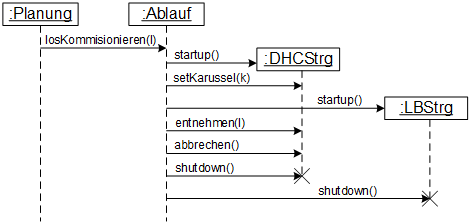
\includegraphics[width=0.75\textwidth]{img/Interaktion1.png}
\caption{\textcolor{blue}{Durch eigene Diagramm ersetzen}}
\label{Interaktion1}
\end{figure}
